\documentclass[12pt,a4paper,twoside]{mwart}
\usepackage[T1]{fontenc}
\usepackage[utf8]{inputenc}
\usepackage[polish]{babel}
\usepackage{polski}
\usepackage{indentfirst}
\usepackage[left=3cm,right=2cm,top=2.5cm,bottom=2.5cm]{geometry}
\usepackage{todonotes}
\usepackage{listings}
\usepackage{float}
\usepackage{hyperref}
\usepackage{dirtree}
\usepackage{fancyhdr}
\usepackage[nottoc,numbib]{tocbibind}
\usepackage{enumitem}
\usepackage{csquotes}
\DeclareQuoteAlias{croatian}{polish}
\usepackage{biblatex}
\addbibresource{References.bib}
\usepackage{url}
\usepackage{amsmath}


\setlength{\parskip}{13pt plus 2pt minus 3pt} %% Odstęp dla paragrafów
%% \linespread{1.15} odstęp pomiędzy liniami?

\newcommand{\makecell}[2][@{}c@{}]{\begin{tabular}{#1}#2\end{tabular}}
\newcommand{\file}[1]{\textbf{\textit{\textcolor{darkgreen}{#1}}}}
\newcommand{\folder}[1]{\textbf{\textit{\textcolor{dodgerblue}{#1}}}}

\pagestyle{fancy}
%% JN: nie jestem pewien czy klasa 'article' z 'openany' ma \markright
%% JN: uproszczenie paginy: tylko autor i tytuł pracy, zamiast tytułu
%%     bieżącego rozdziału.
\renewcommand{\sectionmark}[1]{\markright{#1}}
\fancyhf{}
\fancyhead[LO]{\small \emph{\nouppercase{\leftmark}}}
\fancyhead[RE]{\small \emph{\nouppercase{\rightmark}}}

\cfoot{\fancyplain{}{\thepage}}

% Część odpowiedzialna za styl kodu
% Taken from Lena Herrmann at 
% http://lenaherrmann.net/2010/05/20/javascript-syntax-highlighting-in-the-latex-listings-package
\usepackage{listings}
\usepackage{color}
\definecolor{lightgray}{rgb}{.9,.9,.9}
\definecolor{darkgray}{rgb}{.4,.4,.4}
\definecolor{purple}{rgb}{0.65, 0.12, 0.82}
\definecolor{dodgerblue}{RGB}{28, 134, 238}
\definecolor{darkgreen}{RGB}{0,153,51}
\definecolor{darkOrange}{RGB}{120,30,0}

\lstdefinelanguage{JavaScript}{
  keywords={typeof, new, true, false, catch, function, return, null, try, catch, switch, var, let, if, in, while, do, else, case, break},
  keywordstyle=\color{purple}\bfseries,
  ndkeywords={class, export, boolean, throw, implements, import, this, Math, Float32Array, Array},
  ndkeywordstyle=\color{blue}\bfseries,
  identifierstyle=\color{black},
  sensitive=false,
  comment=[l]{//},
  morecomment=[s]{/*}{*/},
  commentstyle=\color{darkgreen}\ttfamily,
  stringstyle=\color{darkOrange}\ttfamily,
  morestring=[b]',
  morestring=[b]"
}

\lstset{
   language=JavaScript,
   backgroundcolor=\color{lightgray},
   extendedchars=true,
   basicstyle=\footnotesize\ttfamily,
   showstringspaces=false,
   showspaces=false,
   %% JN: jeśli ie odwołuje się do konkretnych linii, to ich numerowanie nie do końca ma sens
   %% JN: jeśli numerowanie linii jest używane do pokazania gdzie linie zostały zawinięte,
   %%     to lepiej użyć mniej agresywnego stylu
   numbers=left,
   numberstyle=\footnotesize,
   numbersep=9pt,
   tabsize=2,
   breaklines=true,
   showtabs=false,
   captionpos=b
}
\setlength{\parindent}{4em}
\setlength {\marginparwidth }{2cm}
\setlength{\parskip}{1em}
\renewcommand{\baselinestretch}{1.5}
\begin{document}

\begin{titlepage}
	\begin{center}
		\large Uniwersytet Mikołaja Kopernika w Toruniu\\
		\large Wydział Matematyki i Informatyki\\
		\vspace{3cm} 
		\large Patryk Bieszke\\
			nr albumu: 273187\\
			informatyka\\
		\vspace{2cm}
		Praca magisterska\\
	
		\vspace{2cm} 
		\huge Generowanie kompozycji muzycznych z użyciem sieci neuronowych\\
	\end{center}
	\hfill
	\begin{minipage}{6cm}
		\vspace{2cm}
		Opiekun pracy dyplomowej\\
		prof. dr hab. Piotr Wiśniewski
	\end{minipage}
	\vspace{3cm}
	\begin{center}
		Toruń 2019\\
	\end{center}
\end{titlepage}


\pagenumbering{gobble}% Remove page numbers (and reset to 1)

\clearpage
\thispagestyle{empty}
\mbox{}

\pagenumbering{arabic}
\tableofcontents 
\clearpage

\setcounter{secnumdepth}{0}
\section{Wstęp}
\label{sec:wstep}

\newpage

\section{Słownik skrótów}
\begin{itemize}
  \item \textbf{FT} - \textit{ang. \textbf{F}ourier \textbf{T}ransform}, pol. Transformata Fouriera
  \item \textbf{DFT} - \textit{ang. \textbf{D}iscrete \textbf{F}ourier \textbf{T}ransform}, pol. Dyskretna Transformata Fouriera
  \item \textbf{FFT} - \textit{ang. \textbf{F}ast \textbf{F}ourier \textbf{T}ransform}, pol. Szybka Transformata Fouriera
  \item \textbf{STFT} - \textit{ang. \textbf{S}hort- \textbf{T}ime \textbf{F}ourier \textbf{T}ransform}, pol. Krótkoczasowa Transformata Fouriera
  \item \textbf{DAW} - \textit{ang. \textbf{D}igital \textbf{A}udio \textbf{W}orkstation}, pol. Cyfrowa Stacja Robocza 
  \item \textbf{MIDI} - \textit{ang. \textbf{M}usical \textbf{I}nstrument \textbf{D}igital \textbf{I}nterface}, pol. Cyfrowy Interfejs Instrumentów Muzycznych
  \item \textbf{AUX} - \textit{ang. \textbf{Aux}iliary}
  \item \textbf{W3C} - \textit{ang. \textbf{W}orld \textbf{W}ide \textbf{W}eb \textbf{C}onsortium}
  \item \textbf{HTML} - \textit{ang. \textbf{H}yper\textbf{t}ext \textbf{M}arkup \textbf{L}anguage}
  \item \textbf{CSS} - \textit{ang.  \textbf{C}ascading \textbf{S}tyle \textbf{S}heets}
  \item \textbf{JS} - \textit{\textbf{J}ava\textbf{S}cript}
  \item \textbf{TS} - \textit{\textbf{T}ype\textbf{S}cript}
  \item \textbf{DOM} - \textit{ang. \textbf{D}ocument \textbf{O}bject \textbf{M}odel}
  \item \textbf{API} - \textit{ang. \textbf{A}pplication \textbf{P}rogramming \textbf{I}nterface}
  \item \textbf{CLI} - \textit{ang. \textbf{C}ommand \textbf{L}ine \textbf{I}nterface}
  \item \textbf{CQRS} - \textit{ang. \textbf{C}ommand \textbf{Q}uery \textbf{R}esponsibility \textbf{S}egregation}
  \item \textbf{URL} - \textit{ang. \textbf{U}niform \textbf{R}esource \textbf{L}ocator }
  \item \textbf{npm} - \textit{ang. \textbf{N}ode \textbf{P}ackage \textbf{M}anager}

\end{itemize}
\newpage
\setcounter{secnumdepth}{2}

\section{Transkrypcja muzyki}
Sygnały akustyczne przechowywane są w postaci binarnych plików dźwiękowych, których zawartością są sygnały foniczne w formie cyfrowej. Sposób, w jaki pliki te przechowują dane jest zdeterminowany przez wiele parametrów, jak kodowanie, które zostało na nich zastosowane, częstotliwość próbkowania, ilość kanałów itp. Istnieje wiele kodowań przeznaczonych do danych dźwiękowych, zarówno nieskompresowanych jak i skompresowanych. Te drugie powstały z myślą o zaoszczędzeniu jak największej ilości pamięci w znaleźć od tego, w jakim stopniu można pójść na kompromis z jakością skompresowanego sygnału \cite[66]{Homerecording:DlaKazdego}. Częstotliwość próbkowania ma również znaczący wpływ na wynikowy rozmiar plików, jak i ilość bitów przeznaczony na pojedyńczy sampel. Wszystkie cechy jakie posiada cyfrowa reprezentacja rzeczywistego dźwięku muszą być wzięte pod uwagę podczas jej przetwarzania.

W kontekście algorytmów generujących muzykę, binarne pliki dźwiękowe nie posiadają efektywnej struktury pozwalającej na trzymanie akustycznych informacji o melodii czy rytmice. Cechy, które można wydobyć ze zdigitalizowanego strumienia audio mogą posłużyć za istotne wskaźniki przy klasyfikacji zbiorów, natomiast kluczowe informacje odnoszące się do struktury kompozycji i harmonii poszczególnych sekcji szukać należy w transkrypcji danego utworu. 

%% z PWN : transkrypcja [łac. transcriptio ‘przepisywanie’], muz. opracowanie utworu muz. na inny niż w oryginale zespół wykonawczy (orkiestracja) lub inny instrument; Pytanie czy rozszerzenie tego znaczenia w języku polskim jest poprawne? także zapisanie utworu inną notacją muz.; transkrybować — zapisywać znakami współcz. notacji muz. utwory zapisane dawnymi systemami notacyjnymi, np. notacją modalną, menzuralną. Po ENG transkrypcja jest zgodna z rozdziałem

\textbf{Transkrypcja muzyki} to proces polegający na zapisaniu danego utworu muzycznego w sposób formalny, taki jak zapis nutowy, z istniejącego zapisu dźwiękowego. Operacja ta wykorzystywana jest do lepszego zrozumienia muzyki i możliwości jej wiernego odtworzenia. Algorytmiczne podejście do tego problemu obejmuje rozpoznanie rytmu i wysokości tonu poprzez analizę zdigitalizowanego sygnału fonicznego. Do zadań tego procesu często zalicza się odseparowanie od siebie poszczególnych instrumentów w danym utworze muzycznym, ponieważ nakładanie się na siebie sygnały odrębnych źródeł stanowi jeden z większych trudności transkrypcji.

Manualna transkrypcja jest procesem skomplikowanym i czasochłonnym nawet dla profesjonalistów z dużym doświadczeniem w tej dziedzinie.

W tym rozdziale przedstawię wciąż nierozwiązany problem automatycznej transkrypcji muzycznej, nakreślając najbardziej problematyczne rejony w oparciu o przykłady już istniejących rozwiązań.  Celem tych rozważań jest przybliżenie ogólnej koncepcji transkrypcji muzycznej, teorii na jakiej się opierają, \todo[inline]{Move somewhere}oraz próba zoptymalizowania części z nich poprzez zrównoleglenie obliczeń wykorzystując kartę graficzną.

\subsection{Jak "działa" muzyka}
Przed dalszymi rozważaniami istotne jest zdefiniowanie terminologii percepcji słuchowej jak i samej muzyki. Muzyka, równoznaczne z utworem muzycznym, są to uporządkowane zbiory dźwięków o odpowiednich wysokościach i głośnościach z zachowaniem odpowiedniego rytmu. Wysokości tych dźwięków są proporcjonalne do częstotliwości wibracji, które zostały wytworzone przez dany instrument lub głos ludzki. Głośność określana jest przy pomocy amplitudy zadanego sygnału akustycznego. Starając się rozłożyć skomplikowaną strukturę utworów muzycznych na rozdzielne części, można wyróżnić cztery rozdzielne składowe, których zbadanie i zinterpretowanie jest przedmiotem algorytmów transkrypcji muzycznej. Są to:
\begin{itemize}
\item Rytm
\item Wysokość tonu
\item Głośność
\item Barwa dźwięku
\end{itemize}
Zapis nutowy utworu jest zdefiniowany w taki sposób, że wszystkie wyżej wymienione cechy są jednoznacznie opisane, z kolei ten jest wystarczającym źródłem informacji dla muzyków aby zagrać dany utwór muzyczny. Zapisane nuty przedstawiają wysokość tonu wraz z długością granego dźwięku i poziomem głośności jaki powinien zostać zastosowany, jego barwę reprezentuje instrument muzyczny do którego odnosi się dany zapis nutowy. 

Klucz w którym został napisany utwór, opisujący harmoniczną podstawę kompozycji jest również bardzo istotną informacją, która dostępna jest na podstawie zapisu nutowego. W praktyce klucz ogranicza dostępne wysokości tonu jakie mogą być zagrane. Wiele kompozycji muzycznych dynamicznie manipuluje kluczem, tworząc mniej statyczne linie melodyczne, co uniemożliwia opieranie transkrypcji o ten parametr.

Zapis nutowy zawiera też informacje o tempie utworu, czyli szybkość z jaką kolejne dźwięki powinny być grane, jak i sygnaturę czasową, która wyznacza bazową strukturę rytmiczną w jakiej dany utwór został napisany. Te dwie informacje składają się na wylistowany wyżej rytm.

Informacją, którą zapis nutowy nie dostarcza jawnie, jest barwa dźwięku. Parametr ten jest ściśle związany z instrumentem, którego dotyczy dany dźwięk. Każde ze źródeł dźwięku cechuje się odrębną barwą, nawet gdy uwzględnić taką samą wysokość i głośność sygnału fonicznego. Problem rozróżniania tej cechy jest związany nie tylko z transkrypcją muzyki, ale i algorytmami identyfikującymi instrumenty poprzez analizę barwy dźwięku.

W dalszej kolejności zostaną pokrótce opisane cztery wymienione wyżej cechy, które są głównym przedmiotem analizy w kierunku transkrypcji muzycznej \cite[63]{Homerecording:DlaKazdego}.
\begin{figure}[H]
  \begin{center}
    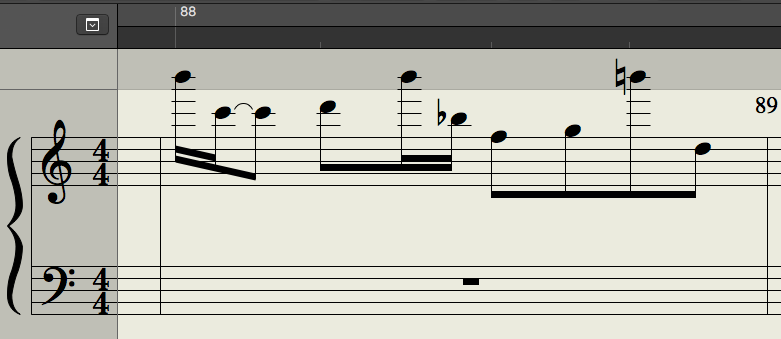
\includegraphics[scale=0.5]{images/pieciolinia_logic.png}
    \caption{Przykład notacji muzycznej wygenerowanej z pliku MIDI w programie Logic Pro X. Widać na nim takie informacje jak metrum czy wysokości i długości granych dźwięków}
  \end{center}
\end{figure}
\subsubsection{Rytm}

W kontekście muzykologii, rytm jest bazową strukturą czasową utworu. Nie można niestety zakładać stałości rytmu na przestrzeni całego utworu, ponieważ powszechną praktyką jest jego modyfikacja w trakcie trwania wykonania w celu uzyskania specyficznych efektów artystycznych. Bardzo częstą praktyką jest na przykład minimalne podnoszenie tempa na czas każdego z refrenów w celu ich wypuklenia na tle całości kompozycji.

Podstawową jednostką rytmiczną jest nuta. Miarą tempa utworu przeniesioną na domenę fizyczną są \textbf{uderzenia na minutę} \textit{(ang. beats per minute, BPM)} oznaczające liczbę ćwierćnut przypadających na jedną minutę. \textbf{Taktem} nazywamy odcinek zapisu muzycznego wizualnie oznaczony pionowymi kreskami. Takty tworzą regularne odcinki czasowe, a ich długość jest zależna od \textbf{metrum}. Metrum jest oznaczeniem metrycznym opisującym ile jakich jednostek mieści się w takcie. Dla przykładu, najpopularniejszym metrum w muzyce pop jest 4/4, co oznacza, że w każdym takcie mieszczą się cztery ćwierć nuty.

\subsubsection{Wysokość tonu}
Wysokością tonu, czy też wysokością dźwięku, nazywana jest częstotliwość drgań źródła fali, czyli ton podstawowy. Zgodnie z zachodnimi standardami tworzenia muzyki, system równomiernie temperowany zakłada skwantowanie spektrum częstotliwości tak zwane półtony, czyli najmniejsze interwały. Każda z tak powstałych muzycznych nut ma przypisaną literę w celu odróżnienia, alfabetycznie od A do G wraz z ewentualnymi podwyższeniami (moll) czy obniżeniami (dur) półtonowymi. Tak nazwane wysokości są grupowane w oktawy, każda zawierająca 12 półtonów. Pełna nazwa granego dźwięku powinna zawierać nazwę literalną wraz z numerem oktawy.

Obowiązujący obecnie strój zakłada referencyjne mierzenie częstotliwości zależnie od wysokości A4, która powinna być równa 440 Hz. Każda oktawa zaczyna się od częstotliwości dwa razy większej od poprzedniej. Standard MIDI\cite[67-71]{Homerecording:LevelUp} mapuje daną częstotliwością bazową na liczbę rzeczywistą odpowiadającą wysokości dźwięku przy pomocy wzoru:
\begin{equation} \label{eq:midi_freq}
p = 69 + 12 * \log{2}(\frac{f}{440 Hz})
\end{equation}

Korzystając ze wzoru ~\ref{eq:midi_freq} dla wielokrotności liczby 440 można uzyskać tabelkę z częstotliwościami kolejnych dźwięków A w oktawach, jak w tabeli \ref{tab:FqMidi}.

\begin{table}[H]
  \begin{center}
    \begin{tabular}{ |c|c|c| } 
    \hline
    p & f & Literalna nazwa wysokości dźwięku\\
    \hline
    33 & 55 & A1\\
    45 & 110 & A2\\
    57 & 220 & A3\\
    69 & 440 & A4\\
    81 & 880 & A5\\
    93 & 1760 & A6\\
    105 & 3520 & A7\\
    \hline
    \end{tabular}
  \end{center}
  \caption{Wysokości kolejnych dźwięków A zgodna ze wzorem ~\ref{eq:midi_freq}}
  \label{tab:FqMidi}
\end{table}


Relacja pomiędzy wysokościami używanych tonów jest ważną informacją przy analizie muzycznej. Mimo dużej ilości możliwych częstotliwości, używane nuty często ograniczane są do podzbiorów według tak zwanych kluczy. Badając rozkład częstotliwości takie informacje mogą znacznie ograniczyć błędy podczas badania sygnału. Należy jednak mieć na uwadze fakt, że nagrany instrument może nie posiadać dokładnie takiej samej częstotliwości jak oczekiwana dla danej wysokości tonu ze względów technicznych. Dodatkowym utrudnieniem są skale które bazują na innych niż zachodnich systemach dobierania wysokości. Równierz z artystycznych względów docelowe częstotliwości generowane przez instrumenty odbiegają od tych przewidzianych przez opisany system. Rozpoznawanie tylko tych sztywnych wysokości tonów mogło by być dużym uproszczeniem w analizie sygnałów fonicznych, lecz jednocześnie znacznie ograniczyłby jej skuteczność \cite[64-65]{Homerecording:DlaKazdego}.

\subsubsection{Głośność}
W notacji muzycznej nie używa się zbyt często słowa "głośność". To co słuchacz odbiera jako siłę dźwięku z punktu widzenia muzyka jest dynamiką granego fragmentu. Większość instrumentów używanych do tworzenia muzyki posiada zdolność wytworzenia zróżnicowanych w sile fal akustycznych. Podstawą skali dynamiki są dwa słowa kluczowe:

\begin{itemize}
  \item \textbf{f} (forte) - głośno
  \item \textbf{p} (piano) - cicho
\end{itemize}

Pomiędzy tymi stopniami są kroki pośrednie, odpowiednio mezzo-forte (dość głośność) i mezzo-piano (dość cicho). Poza czterema wymienionymi przypadkami dostępne są również skrajności odpowiadające za bardzo głośny (odpowiednio - cichy) i możliwie najgłośniejszy (odpowiednio - najcichszy) odcień dynamiki. 

Z punktu widzenia algorytmicznej analizy muzyki problematyczne są dynamiki zwane crescendo i diminuendo. Odpowiadają one za kolejno stopniowe wzmacnianie i stopniowe osłabianie natężenia dynamiki. Łatwo jest pomylić takie zabiegi z innymi cechami sygnału audio.

Warto też wspomnieć o technice zwanej \textit{tremolo}, która określa artykulacje  grania wielu dźwięków o tej samej wysokości z różną dynamiką. Analizując sygnał łatwo jest pomylić kolejne uderzenia tremolo z zagraniem nowych nut.

Z praktycznego punktu widzenia głośność w plikach muzycznych jest zdeterminowana przez to, jak dany utwór został wyprodukowany. W procesie nagrywania ogromne znaczenia ma położenie i rodzaj mikrofonu, jak i otoczenie w którym rejestrowany jest dźwięk. Charakterystyka niektórych powierzchni może sprawić, że fałszywie cichsze częstotliwości będą wychodziły na przód nagrania. Kompresja dynamiki utworu jest powrzechną praktyką podczas miksowania i masterowania utworów. Dzieje się tak ponieważ ludzie impulsywnie uważają głośniejsze utwory za lepsze, co doprowadziło rynek muzyczny do produkowania utworów o niemal stałej dynamice głośności. Choć temat ten jest w trakcie regulacji, przez między innymi wprowadzenie ograniczeń dynamiki na podstawie jednostki LUFS danego utworu, dokładne analizowanie głośności wielu istniejących nagrań może doprowadzić do nieprawdziwych wniosków.

\subsubsection{Barwa dźwięku}
Barwa dźwięku (inaczej tembr) jest cechą odwołującą się harmonicznej domeny sygnału fonicznego. Pozwala ona odróżnić od siebie dźwięki o tej samej głośności i wysokości grane na różnych instrumentach. Silne tony harmoniczne danej barwy sprawiają, że dźwięk jest bardziej wyrazisty. W przeciwnym wypadku, gdy siła tonów harmonicznych jest mała, sygnał staje się bardziej rozmyty dla odbiorcy. Barwa dźwięku jest zależna od amplitudy poszczególnych tonów harmonicznych, ich rozkładu w widmie jak i samej struktury tego widma. Jest to dobrze widoczne na rysunku \ref{fig:spektrogram}.

\begin{figure}[t]
  \begin{center}
  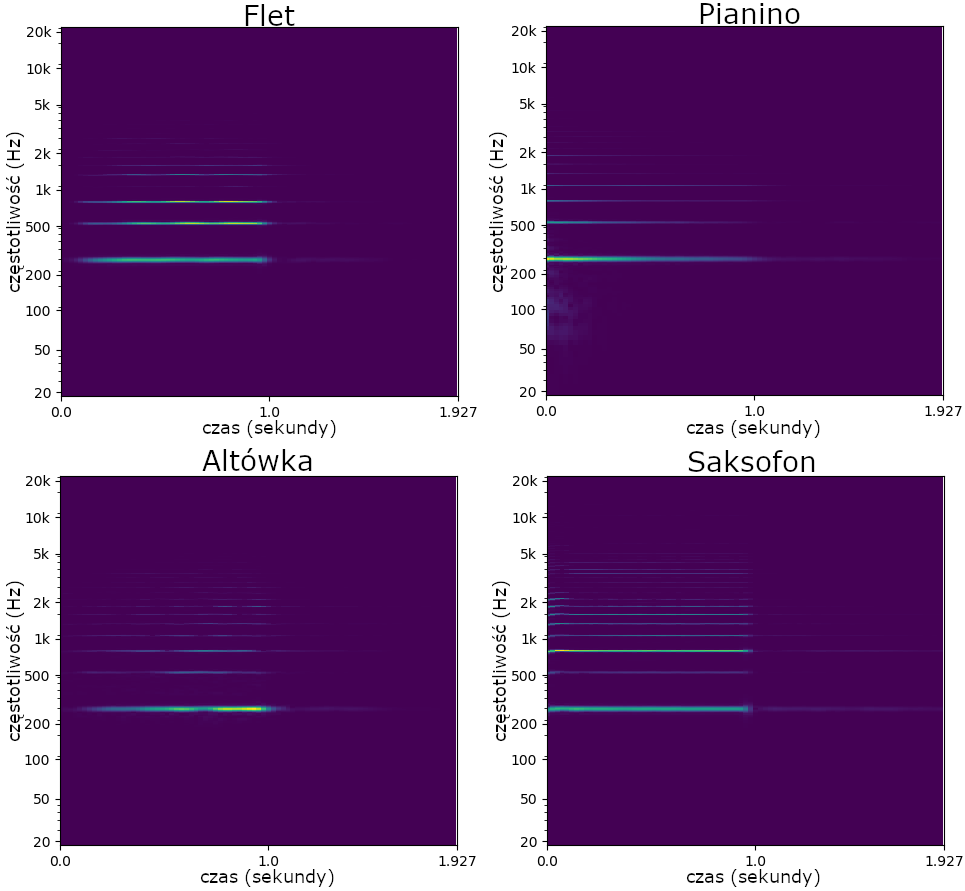
\includegraphics[scale=1.35]{images/spectogram_instruments.png}\\
  \caption{Spektrogramy dźwięku C3 (130.81Hz) grane na różnych instrumentach pokazują różnice w harmonicznych każdego z wykonań. Wykresy zostały wygenerowane przy pomocy funkcji z sekcji "Funkcje pomocnicze". Więcej informacji w sekcji ~\ref{sec:implementacja}}
  \label{fig:spektrogram}
  \end{center}
\end{figure}

Ułożenie tonów harmonicznych jest zintegrowane z harmonią pomiędzy różnymi granymi nutami. Gdy dwa dźwięki są grane w tym samym czasie, nakładające się na siebie harmoniczne sprawiają, że dźwięk brzmi pozornie spójnie. Generuje to dodatkowe komplikacje dla algorytmów wykrywających wysokość tonów, które muszą odseparować nakładające się na siebie nuty.

Barwa dźwięku nie jest stała w czasie. Wysokie harmoniczne szybciej cichną w porównaniu do tych niższych. Sprawia to, że nie tylko ogólna głośność jest mniejsza, ale i barwa ulega modyfikacji. Dla instrumentów dętych czy skrzypiec cechy jak wysokość tonu, głośność i barwa pozostają relatywnie stałe przez cały okres grania nuty, natomiast dźwięk pianina rozmywa się w czasie. Ta cecha barwy dźwięku musi zostać zaadresowana przy próbie dokładnej analizy sygnału fonicznego \cite[64-65]{Homerecording:DlaKazdego}.

Znaczącym pojęciem przy omawianiu barwy dźwięku jest \textbf{formant}. Formantem nazywane jest pasmo częstotliwości, w którego obrębie częstotliwości harmoniczne są wzmocnione względem pozostałych częstotliwości danego sygnału. Formanty mogą sprawić, że harmoniczne będą miały większą amplitudę niż częstotliwość fundamentalna. Istnienie tego zjawiska fonicznego uniemożliwia poprawność podejścia, w którym jako częstotliwość fundamentalna wybierana była by ta, o największej amplitudzie w analizowanym oknie \cite[62-63]{BarwaDzwieku:Formant}.
\todo[inline]{Czy mogę użyć książki której nawet nie mogę znależć on-line tylko jako referencja w innej pozycji?}

\subsection{Transformacja Fouriera}\label{sec:TF}
Z racji tego, że analiza surowych plików dźwiękowych jest wysoce skomplikowana i niepraktyczna w kontekście przetwarzania sygnałów, kluczowym jest przeniesienie tego problemu na płaszczyznę częstotliwości. Do tego celu powszechnie używane jest narzedzie matematyczne zwane \textbf{transformacją fouriera}. Zastosowania tej funkcji są wysoce różnorodne dzięki jej uniwersalności, my jednak skupimy się na benefitach jakie przynosi ona w sferze przetwarzania sygnałów. Transformata ta opiera się na założeniu, że każdą okresową krzywą można zapisać w postaci sumy składowych sinusoidalnych o różnych częstotliwościach. Funkcja ta przekształca sygnału z dziedziny czasu na dziedzinę częstotliwości, co daje zarays tego jak rozłożona jest częstotliwość poszczególnych częstotliwości w analizowanych danych. Transformata zadana jest wzorem:

\begin{equation} \label{fourier-base}
F(f) = \int_{\infty}^{-\infty}\textit{f}(t)e^ {-j2\pi ft}\mathrm{d}x
\end{equation}

Gdzie F(f) nazywane jest transformatą Fouriera f(t) lub widmem częstotliwościowym \cite{TransformacjaFourieraWroc}\cite{TransformacjaFourieraAgh}.

\subsubsection{Dyskretna transformacja Fouriera} \label{sec-DTF}

Przyglądając się własnościom tranformacji Fouriera łatwo zauważyć, że jednym z założeń jest aby f(t)\ref{fourier-base} była funkcją ciągłą na przedziale od minus nieskończoności do nieskończoności, co przekłada się na transformatę w tym zbiorze właśnie. Z praktycznego punktu widzenia nieskończone granice sumy są niemożliwe do zrealizowania, co za tym idzie, w przypadku analizy sygnału sonicznego warunek ten jest również niespełnialny, ponieważ przetwarzane są tylko ograniczone odcinki krzywej, więc granice są zawsze skończone. W celach analitycznych na utworach muzycznych, zwłaszcza w kontekście transkrypcji muzycznej, transformata całego utworu nie jest szczególnie przydatna. Potrzebne do tego celu będzie podzielenie analizowanych danych na krótkie próbki, których transformata przyniesie dalsze wnioski.\cite{TransformacjaFourieraWroc}\cite{TransformacjaFourieraelektronikab2b}

\textbf{Dyskretna transformata Fouriera (DTF)} jest narzędziem matematycznym analogicznym do podstawowej transformaty Fouriera, lecz przeznaczonym do analizowania sygnału dyskretnego $x(n)$ o okresie $N$:
\begin{equation} \label{fourier-cykl}
  x(n) = x(n + mN)
\end{equation}
pozwalającym na analize pojedyńzczego okresu zadanego sygnału. Własność ta jest szczególnie przydatna przy komputerowej analizie sygnałów, w tym fonicznych. Jest to transformacja zawsze odwracalna. 

DTF zakłada wyznaczenie iloczynu sygnału i okna prostokątnego, które to jest wycinkiem krzywej sygnału podlegającym analizie. W związku z cyklicznością zakładanego sygnału (\ref{fourier-cykl}) przyjmuje się, że analizowany sygnał jest okresowy z okresem równym $N$, co implikuje obliczenie dokładnie N składowych charmonicznych analizowanych danych (N różnych częstotliwości). Dyskretny czas, częstotliwość i skończona liczba próbek zadanego sygnału sprowadza omawianą transformacje do funkcji w pełni dyskretnej. Wynik dyskretyzacji TF jest następującą parą równań:
\begin{equation} \label{DTF-equation1}
  X(k) = \frac{1}{N}\sum_{n = 0}^{N-1} x(n)e^{-j \frac{2 \pi} {N} kn},  k = 0, 1, 2,..., N-1
\end{equation}
\begin{equation} \label{DTF-equation2}
  x(n) = \sum_{k = 0}^{N-1} X(k)e^{j \frac{2 \pi} {N} kn}, n = 0, 1,  2,...,N-1
\end{equation}

Wynikiem transformacji będzie N liczb odpowiadających kolejno amplitudzie i fazie sinusoid od $- \frac{1}{2} \Delta $ do $\frac{1}{2} \Delta $, gdzie $\Delta$ jest częstotliwością próbkowania, w rozdzielczości $\frac{1}{N} \Delta$. Częstotliwości są ustalone przez częstotliwość próbkowania oraz liczbę próbek w oknie \cite[198 - 200, 204-206]{CyfrowePrzetwarzanieSygnalowOdTeoriiDoZastosowan}.

\subsubsection{Szybka transformacja Fouriera} \label{sec-FFT}
Wydawało by się, że posiadając narzędzie tak potężne jak transformacja DTF omawiana w sekcji \ref{sec-DTF} jest wystarczająca do wykonania wszelkich analitycznych przekształceń. Problem jednak pojawia się w praktyce, i jest nim efektywność algorytmu. W swojej czystej formie transformata Fouriera $F_n$ wymaga zliczenia wszystkich wartości od $h_0$ do $h_{N-1}$ dla każdej z częstotliwości $n$, co oznacza że złożoność obliczeniowa dla N danych wynosi $O(N^2)$, co jest zbyt dużym obciążeniem nawet dla współczesnych komputerów do analizy dużego zbioru danych. Istnieje wiele metod optymalizacji numerycznych równań \ref{DTF-equation1} i \ref{DTF-equation2} zmniejszających złożoność obliczeniową do conajwyżej $O(N log_2 N)$. Algorytmy te nazywają się \textbf{szybkimi transformacjami Fouriera (FFT)} i to z nich korzysta się powrzechnie przy cyfrowej analizie sygnałów.

Isnieje wiele algorytmów zaliczających się do grupy algorytmów FFT. Popularnym algorytmem jest algorytm \textbf{Cooleya-Tukeya} w formie \textbf{Radix-2} (FFT o podstawie 2). Korzysta on z metodologii \textit{dziel i zwyciężaj}, dzieląc próbkę danych wielkości $N$ na dwie oddzielne przeplatane grupy wielkości $N_1$ i $N_2$ $(N_1 + N_2 = N)$ o indeksach parzystych (0, 2, 4, ...) i nieparzystych (1, 3, 5, ...) wykonując DFT na każdym ze zbiorów, a następnie odtworzenie kompletnego widma sygnału z otrzymanych wyników częściowych. W uproszczeniu algorytm wygląda następująco:
\begin{enumerate}
  \item{Zmiana kolejności próbek. Próbki dzielone są rekurencyjnie na próbki o indeksach parzystych i nieparzystych tworząc przeplatane ciągi, aż do uzyskania zbiorów dwuelementowych.}
  \item{Na każdym z uzyskanych zbiorów wykonuje się DFT, czyli łącznie $\frac{N}{2}$ dwupunktowych DFT.}
  \item{Proces składania widm powtażamy tak, że dwuprążkowe widma składane są w czteroprążkowe, czteroprążkowe w ośmioprążkowe itd., do momentu, w którym odtworzone zostanie widmo N-prążkowe, czyli kompletne widma sygnału.}
\end{enumerate}
Co daje łączną ilość etapów operacji równą $\log_2 N$. \cite[241-252]{CyfrowePrzetwarzanieSygnalowOdTeoriiDoZastosowan}

\subsubsection{Krótkoczasowa transformacja Fouriera}\label{sec:STFT}
W rozdziale \ref{sec:TF} przeanalizowaliśmy działanie i podstawowe odmiany algorytmu transfromacji Fouriera, jednak aby można było wykorzystać w pełni to narzędzie przy analizie utworów muzycznych niezbędne jest wprowadzenie metody czasowo-częstotliwościowej TF. \textbf{Krótkoczasowa transformacja Fouriera (STFT)} jest przeznaczona do operowania na małym oknie analizowanej krzywej. Podczas analizy i syntezy wykorzystywane jest pojedyńcze okno. Definicja STFT w dziedzinie czasu i częstotliwości wygląda następująco:
\begin{equation} \label{STFT-equation1}
  STFT^{T}_{x}(t,f) =\int_{-\infty}^{+\infty} x(\tau)\gamma^{*}(\tau - t)e^{-j2\pi f\tau}  \,\mathrm{d}\tau
\end{equation}
\begin{equation} \label{STFT-equation2}
  STFT^{F}_{x}(t,f) = e^{-j2\pi ft} \int_{-\infty}^{+\infty} X(v) \Gamma^{*} (v-f) e^{j2\pi vt} {d}v
\end{equation}

W równaniu \ref{STFT-equation1} funkcja $\gamma(x)$ oznacza czasowe okno obserwacji, zaś $\Gamma(f)$ jest jej widmem Fouriera. Rozmiar okna dopierany jest zgodnie z zapotrzebowaniem. Dla przykładu, podczas detekcji mowy okno powinno być jak najmniejsze, poniważ dynamika tonacji przy każdym słowie jest bardzo wysoka, i w celu odpowiedniego przeanalizowania wypowiedzi wysamplowane fragmenty, które poddawane są pokolei STFT powinny być jak najmniejsze, aby nie umkneły nawet najdrobniejsze zmiany tonu\cite{MultipleFundamentalFrequencyEstimation}.

Równania \ref{STFT-equation1} oraz \ref{STFT-equation2} noszą metody "przesuwającego się okna" MWM (\textit{ang. Moving Window Method}) w dziedzinie czasowej (\ref{STFT-equation1}) lub częstotliwościowej (\ref{STFT-equation2}). STFT wykonywane na dziedzinie czasowej sprowadza się do wykonywania przekształcenia Fouriera na kolejnych fragmentach wysamplowanego sygnału poprzez przesuwanie okna $\gamma(x)$. W dziedzinie częstotliwościowej algorytm ten:
\begin{enumerate}
  \item odwrotnemu przekształceniu Fouriera fragmentu widma sygnału,
  \item przesunięciu w częstotliwości sygnału czasowego otrzymanego z pkt. 1 do częstotliwości zerowej.
\end{enumerate}
\cite[455-458]{CyfrowePrzetwarzanieSygnalowOdTeoriiDoZastosowan}

Bardzo małe okna czasowe kładą większy nacisk na domenę czasową niż częstotliwościową. Dla algorytmów wykrywających tonacje muzyki precyzja w częstotliwości jest dużo bardziej istotna niż precyzja w czasie. Technika, która pozytywnie wpływa na dokładność w obu tych płaszczyznach, zakłada nakładanie na siebie okna, przesuwajac je mniej niż jego właściwą szerokość. W zależności od tego jak mocno okno się na siebie nakłada proporcjonalnie rośnie koszt obliczeniowy tego algorytmu. \cite{WindowChoiceStrategiesSTFT}

W momęcie gdy w algorytmie okno nakłada się na siebie znacząca porcja danych jest zduplikowana. Aby zminimalizować ten negatywny efekt funkcja okna jest specjalnie dostosowywana. W ogólności, funkcja okna wydobywa odpowiednie wartości wewnątrz jej zakresie (w oknie) i stałą wartość (zazwyczaj jest to zero) wszędzie poza wyznaczonym zasięgu. Dla okien czasowych można stosować wiele różnych funkcji matematycznych. W tabeli \ref{tab:definicjeOkien} przedstawione są funkcje, które mogą być użyte jako okna czasowe wraz z ich analityczbymi wzorami widm $W(\omega)$\cite[103, 106]{CyfrowePrzetwarzanieSygnalowOdTeoriiDoZastosowan}\cite{RobustMethodOfMeasurmentOfFundamentalFq}.
\begin{table}[H]
  \begin{center}
    \begin{tabular}{ |c|c|c| } 
    \hline
    Nazwa funkcji & $w(t)$ & $W(\omega)$\\
    \hline
    Prostokątna & $p_T (t) = \left\{
      \begin{array}{ll}
        1 \text{ dla } |t| <= T\\
        0 \text{ dla } |t| > T\\
      \end{array}
    \right.  $ & $2\frac{\sin \omega T}{\omega}$\\
    \hline
    Trójkątne (Bartletta) & $q_T = \left\{
      \begin{array}{ll}
        1-|t|/T \text{ dla } |t| <= T\\
        0 \text{ dla } |t| > T\\
      \end{array}
    \right. $ & $T[\frac{\sin(\omega T / 2)}{\omega T/2}]^2$\\
    \hline
    Hanninga (Hanna) & $[0,5 + 0,5 \cos(\pi t / T)]p_T (t)$ & 
    $\frac{\pi^2 \sin(\omega T))}{\omega(\pi^2 - T^2 \omega^2)}$\\
    \hline
    Hamminga & $[0,54 + 0,46\cos(\pi t/T)]p_T (t)$ & 
    $\frac{(1,08\pi^2 - 0,16T^2\omega^2)}{\omega(\pi^2 - T^2 \omega^2))}\sin(\omega T)$\\
    \hline
    \end{tabular}
  \end{center}
  \caption{Definicje funkcji okien czasowych $w(t)$ i analityczne wzory ich widm $W(\omega)$}
  \label{tab:definicjeOkien}
\end{table}
\begin{figure}[H]
  \begin{center}
    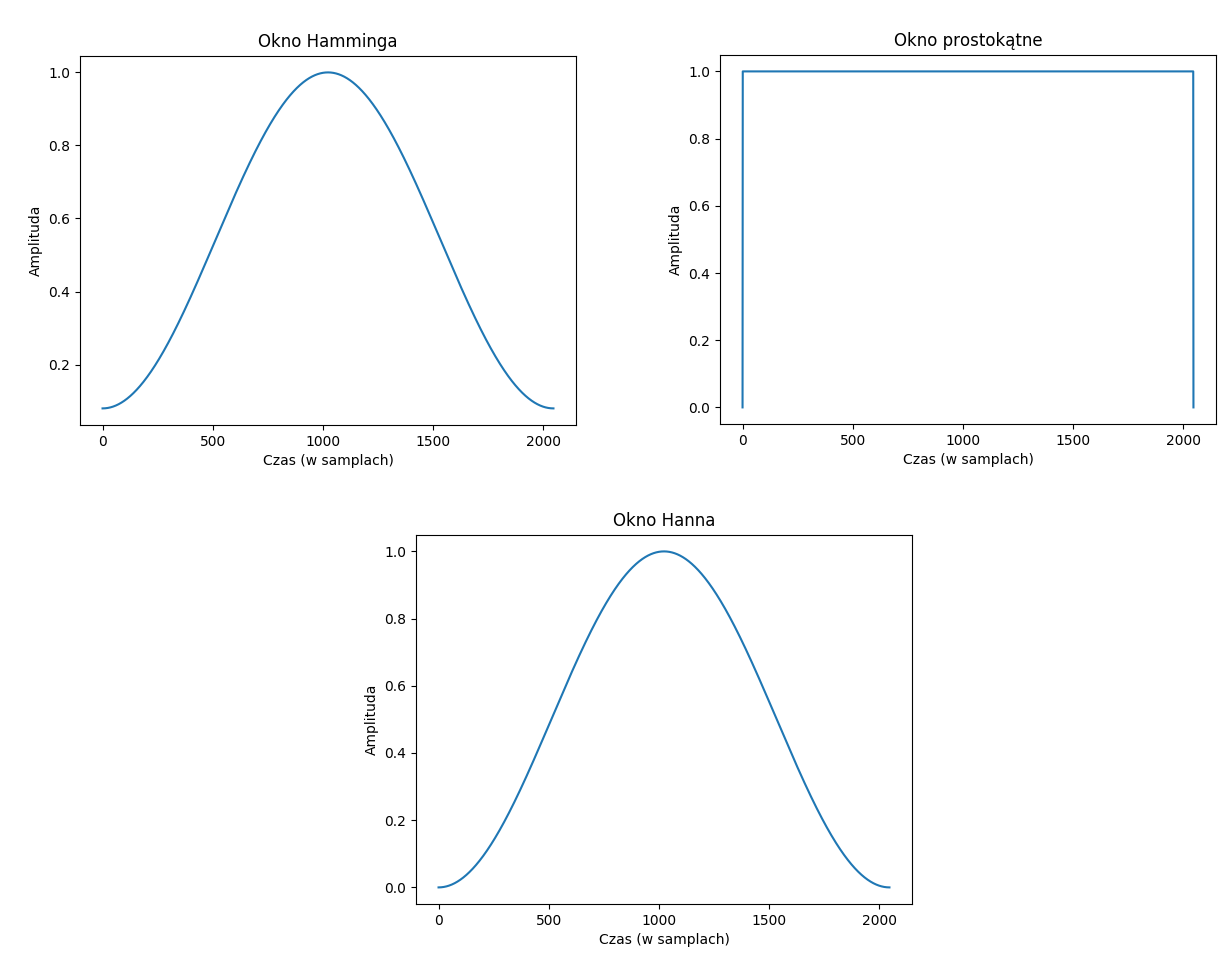
\includegraphics[scale=1.4]{images/WindowFunctions.png}
    \caption{Przykład funkcji okna czasowego dla ramki audio zawierającej 2048 sampli}
  \end{center}
\end{figure}
\newpage

\subsection{Estymacja składowej fundamentalnej F0}
\newpage

\subsection{Estymacja wielotonowa}
Zaimplementowana transkrypcja przez harmoniczne

\newpage
\section{Klasyfikacja muzyki}
\cite{DBLP:journals/corr/abs-1708-03535}\cite{DBLP:journals/corr/XiongDHSSSYZ16a}
\todo[inline]{Najprawdopodobniej rozdział do usunięcia, lub do czysto teoretycznego opisu}

\section{Generowanie muzyki}
\begin{figure}[H]
  \begin{center}
    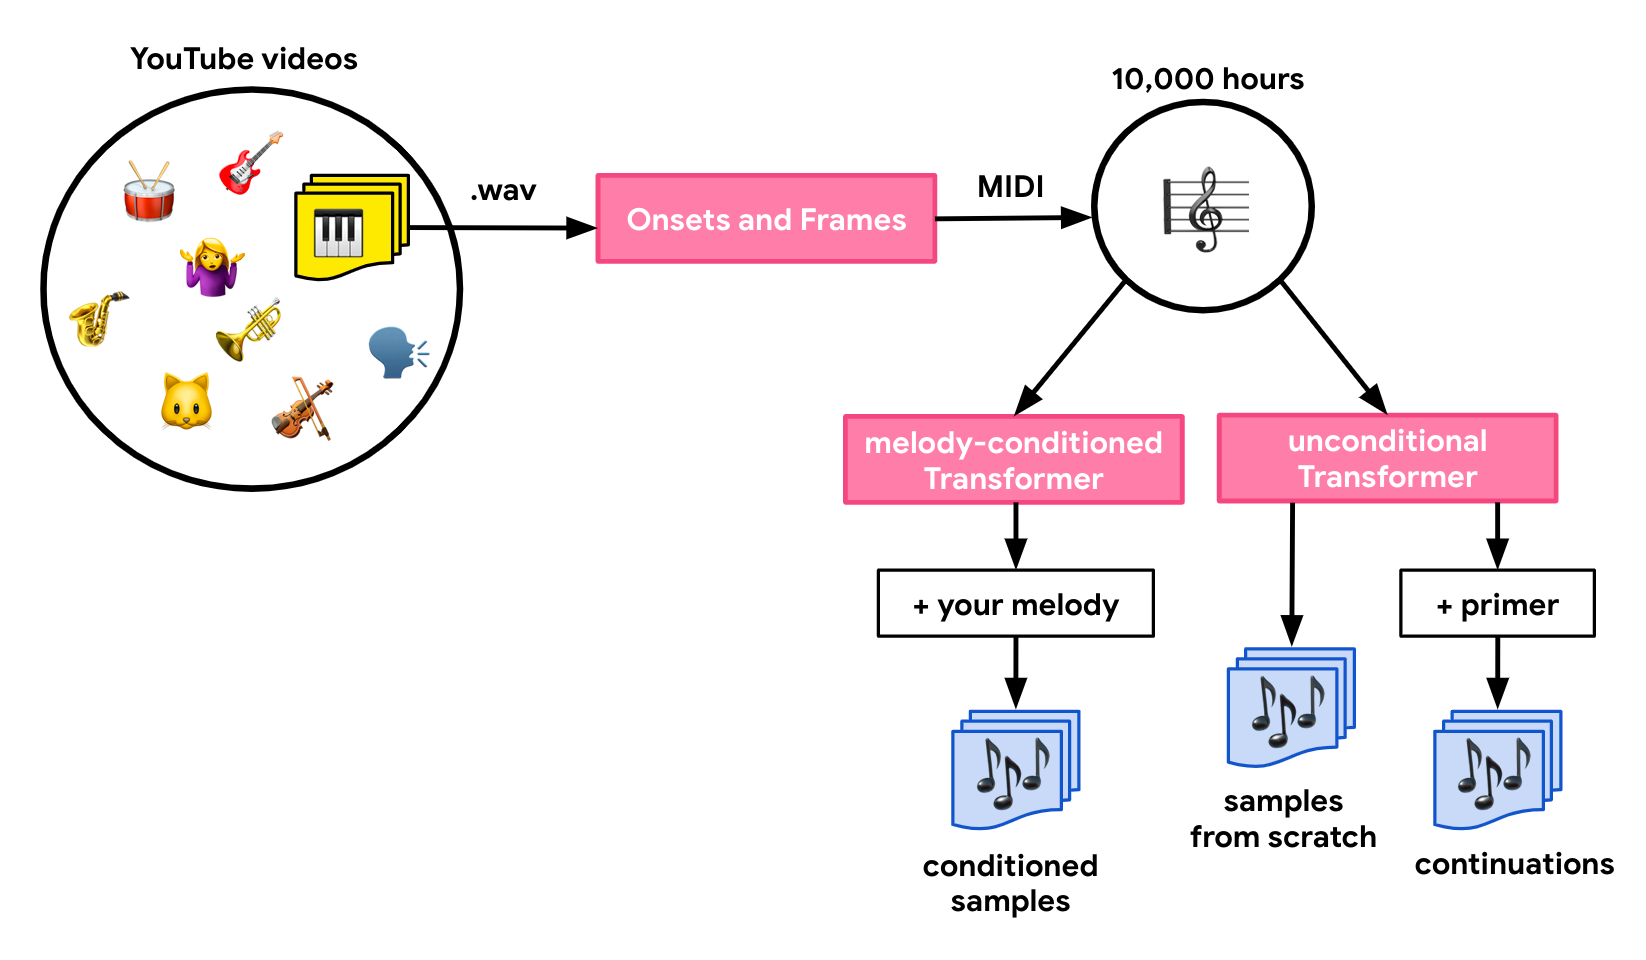
\includegraphics[scale=0.25]{images/pianoTransformerDiagram.png}
    \caption{z https://magenta.tensorflow.org/piano-transformer, diagram przedstawiający działanie modelu Music Transformer. Do wyszukania odpowiednich klipów z YouTube został wykorzystany model AudioSet \cite{audioSet} do wyodrębnienia audio jedynie z pianinem.}
  \end{center}
\end{figure}
\todo[inline]{Czy można tak używać grafiki z innych stron? Czy odniesienie do strony w bibliografi jest prawidłowe?}

\cite{DBLP:journals/corr/abs-1809-04281}\cite{DBLP:journals/corr/VaswaniSPUJGKP17}
\cite{DBLP:journals/corr/HuangW16}
\cite{DBLP:journals/corr/abs-1810-12247}
\newpage

\section{Implementacja}
\label{sec:implementacja}
~\ref{eq:midi_freq}
\subsection{Funkcje pomocnicze}
\newpage
\subsection{Transpilacja}
\begin{figure}[H]
  \begin{center}
    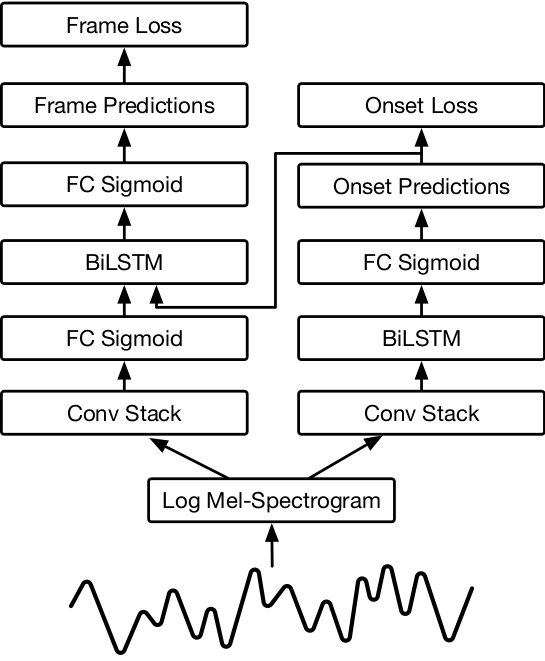
\includegraphics[scale=0.8]{images/architekturaSieciOnesetsFrames.png}
    \caption{z https://magenta.tensorflow.org/onsets-frames, diagram przedstawiający architekture sieci Onesets and Frames.}
  \end{center}
\end{figure}
\cite{DBLP:journals/corr/LuongPM15}
\newpage

\subsection{Składowanie danych}
\newpage

\subsection{Generowanie muzyki}
\newpage
\subsection{Interfejs}
\cite{reactWDzialaniu}\cite{tsDocumentation}
\newpage
\section{Zakończenie}
\newpage


\printbibliography

\end{document}  
